\chapter{Methodology}\label{chapter:Methodology}
This chapter proposes three different signal distribution networks that overcome the restrictions of the placement and routing algorithm, ortho, which was reviewed as the state of the art in chapter \ref{chapter:SotA}. Specifically, an ordering network, a majority gate network, and a sequential distribution network are introduced.

The placement and routing algorithm, ortho, has been shown to have limitations, but it still possesses a powerful placement and routing procedure. To overcome these limitations, it is proposed to maintain the foundation of the algorithm while incorporating new functionalities. These new functionalities often result in irregularities, such as in the clocking or routing, and the goal of the proposed signal distribution networks is to redistribute signals on the layout in a way that these irregular parts align with the regular placement and routing while still satisfying all design constraints. In this way, the algorithm can still function in a similar manner as ortho. However, the underlying logic network and the placement and routing must also be modified to incorporate the desired functionalities, adding complexity to the preprocessing and algorithm.

Since ortho is restricted to the use of only 2DD-Wave clocking, the signal distribution networks must have the ability to change the clocking in the layout to implement their respective functionalities. Therefore, the implementation of these networks must be done with care and synchronization constraints must be closely considered.

The ordering distribution network is discussed first, which aims to reduce the area in the input region of the layout. Afterwards, the networks used for implementing majority gates and sequential parts are discussed and analyzed.

\section{Ordering Distribution Network}

\begin{figure}
	\centering
	\begin{tikzpicture}[node distance={2cm and 2cm}, thick, main/.style = {draw, rectangle}] 
		\node[fit={(0,0) (8, 8)}, inner sep=0pt, draw=black, thick] (frame) {};
		\node[fit={(1.5,0) (6.5, 8)}, inner sep=0pt, draw=black, thick, fill=cyan] (logic) {Combinational logic};
		\node[fit={(0,6.5) (1.5, 8)}, inner sep=0pt, draw=black, thick, fill=TUMGray] (PIs) {ordered \\ PIs};
		\node[fit={(6.5,0) (8, 8)}, inner sep=0pt, draw=black, thick, fill=TUMGray] (POs) {POs};
		
		\draw[] (1, 6.5) -- (6.5, 6.5);
		
		\draw (4,7.25) node [align=left] {Area used to place \\ the ordering network};
		
		
	\end{tikzpicture} 
	\caption{Scheme of area usage in the Ordering Distribution Network} \label{fig:ordering_scheme}
\end{figure}

Looking again at the resulting layout of a 2:1 MUX designed by ortho in \ref{fig:ortho_mux_21}, it can be observed that in the first few rows, where the primary inputs are placed, no other gates are placed, as the space has been reserved for rewiring to resolve conflicts. The idea of the ordering distribution network is to order and place inputs in a way that wire crossings can be minimized and gates can be placed in the input area to save space. Additionally, after reordering the primary inputs (PIs), the remaining logic network is ordered topologically, so that the improvements following the ordering of the PIs can be applied to the entire network. To allow the usage of the input area, the ordering network must resolve conflicts in a different way.

Recalling the pseudo-code from the ortho algorithm \ref{alg:ortho}, an input has a conflict when it is colored south, which would lead the routing to wire over the other inputs in the same column, which is not allowed. This means that the area overhead in the input region is highly dependent on the coloring assigned to the outgoing edges of the inputs. Line $3$ of the pseudocode, which invokes the coloring algorithm, finds a valid but not an optimal coloring for the given logic network. Unfortunately, due to the algorithm's nature, it often assigns the color south to edges connected to PIs resulting in conflicts and area overhead.

Therefore, two preprocessing steps are introduced. In the first step the PIs are ordered, depending on their outgoing edges, allowing PIs connected with the same gates to be placed near each other reducing wire expenses and crossings. Secondly, the coloring in the input region of the logic network is improved to prevent excess wiring. To enable the use of the preprocessing steps, also new rule for edges colored south is introduced, making the rewiring redundant. This rule is found to be effective not only inside the conflicting input area but for the whole layout.

To examine the concept, it is necessary to first identify the portions of the logic network that belong to the ordering distribution network. This can be determined by examining the nodes that are placed in the input area. These include nodes that are directly connected to the primary inputs (PIs) and nodes that are connected to these nodes and colored east. For the network, all nodes that are successively connected, starting at each PI and ending at the first node with two fan-ins, are considered. Once these nodes are placed correctly, all conflicts are resolved, and the ortho algorithm can function as intended. The respective ordering and coloring should then be discussed, starting with the different gates inputs can be connected to.

\begin{algorithm}[H]
	\vdots
	
	\begin{algorithmic}
		\State Convert $N$ to a 3-graph by substitution and balance inverters at fan-out nodes
		\State Order primary input nodes
		\State \vdots
		\State Generate \textbf{conditional} direction assignment $d : \Delta \rightarrow \{east, south\}$ and subdivide signals if necessary
		\State Compute topological ordering $v_1, . . . , v_i \in N$
		\State Extend $L$ by one column and reserve it for primary inputs
		\ForAll {vertex $v_1, ..., v_i \in N $ with at most two incoming signals $\sigma_1, \sigma_2$}
		\If{vertex $v$ is terminal/primary input}
		\State Extend $L$ by one row
		\State Place v at position $(0, h - 1)$
		\ElsIf{$d(\sigma_1) = d(\sigma_2) = east$}
		\State \vdots
		\ElsIf { signals are labeled $south$}
		\If{\textbf{not} root node exists}
		\State Extend $L$ by one row
		\EndIf
		\State $w_p \leftarrow$ max. horizontal position of v's predecessors
		\State Place v at position $(w _p, h - 1)$
		\EndIf
		
		\EndFor
		\State \vdots \\
		\Return $L$
	\end{algorithmic}
	\caption{Ortho changes with ordering distribution network}\label{alg:input_network}
\end{algorithm}

For the ordering, primary inputs (PIs) connected to the same two-fanin gate are placed consecutively, minimizing the routing distance and reducing the probability of wire crossings. In addition to ordering, a valid coloring must also be found for all nodes in the ordering distribution network. This requires consideration of all types of nodes connected to PIs.

The direction assignment for one-fanin nodes, including inverters and fan-out nodes, can be chosen arbitrarily as the primary input to which they are connected has only one outgoing edge, resulting in no dependencies. In this case, the non-conflicting east assignment can always be chosen. When examining two-input logic gates such as AND and OR gates, the coloring can only be chosen arbitrarily if both input nodes are primary inputs, again allowing for the non-conflicting assignment of east. In all other cases, the direction assignment must consider the coloring of the other incoming edge of the gate. To determine dependencies, all one-fanin nodes must first be colored, including inverters and fan-outs.

Regarding fan-outs, following the coloring rules, the two outgoing edges need to be colored in different directions, so that the fan-out gates placed into the network have one output assigned with color $east$ and one output assigned with color $south$. Considering that the second coloring constraint requires both incoming edge of the gate connected to the edge colored $south$, also to be colored $south$, and the second incoming edge being connected to a PI, we can see that a conditional coloring alone is not powerful enough to resolve all conflicts. For this case a new placement rule for the $south$ coloring is introduced in order to preserve the direction assignment rules but still resolve the conflict between primary inputs. The original algorithm part (lines 14-22) handling the placement of nodes based on their coloring makes sure that every gate placed $east$ occupies a new column and every node colored $south$ occupies a new row. These placement rules allow every gate to be placed without interfering with other gates, but the rules have been found to be too restrictive, allowing the following placement rule for $south$. If a node is labeled south and its predecessor, which has the lower horizontal position \textbf{also} has the higher vertical position, it is called \textit{root node} and the layout is \textbf{not} extended by a row while the gate is still in position $(w_p, h-1)$. Following this rule the gate is now placed in the same row as its root node and the same column as the predecessor with the higher x-coordinate. If we apply this to a two-input gate in the ordering distribution network with a primary input and a fan-out node as predecessors, the primary input is always the root node due to the ordering and new coloring. Thus, the new rule allows the two-input gate connected to the primary input colored $south$ and the fan-out node to be placed in the same column as the primary input, resulting in no conflict because the node is not \textit{actually} placed south of its predecessors. It was found that this rule could not only be utilized for resolving PI conflicts, but also for the general $south$ placement in the algorithm with one exception. Though, considering a fan-out node to be the root node, the coloring would wire both the eastern and the southern colored outgoing edges onto the same row, yielding a conflict. For this case the new rule is not applied and this case is excluded for the input area through the ordering. The resulting pseudo-code snippets replacing the used code are shown in algorithm \ref{alg:input_network}. Also it has to be considered that the conditional coloring in the distribution network still needs to include helping nodes e.g. when three fan-out nodes are connected to the same nodes. Also before the coloring, first the input nodes need to be ordered according to the ideas presented. Thus, primary input nodes connected to fan-out nodes are placed first and then the primary input nodes, which are connected to the outgoing edges of the fan-out nodes are placed. This is done to reduce the distance between coherent gates and therefore also the number of wire crossings. Afterwards primary inputs directly connected to a gate which has its other incoming edge connected to a second primary input are placed. Finally all input nodes, which are not connected to the rest of the ordering distribution network are placed arbitrarily and the logic network is topologically ordered according to the new order of the primary inputs.


\begin{figure}
	\centering
	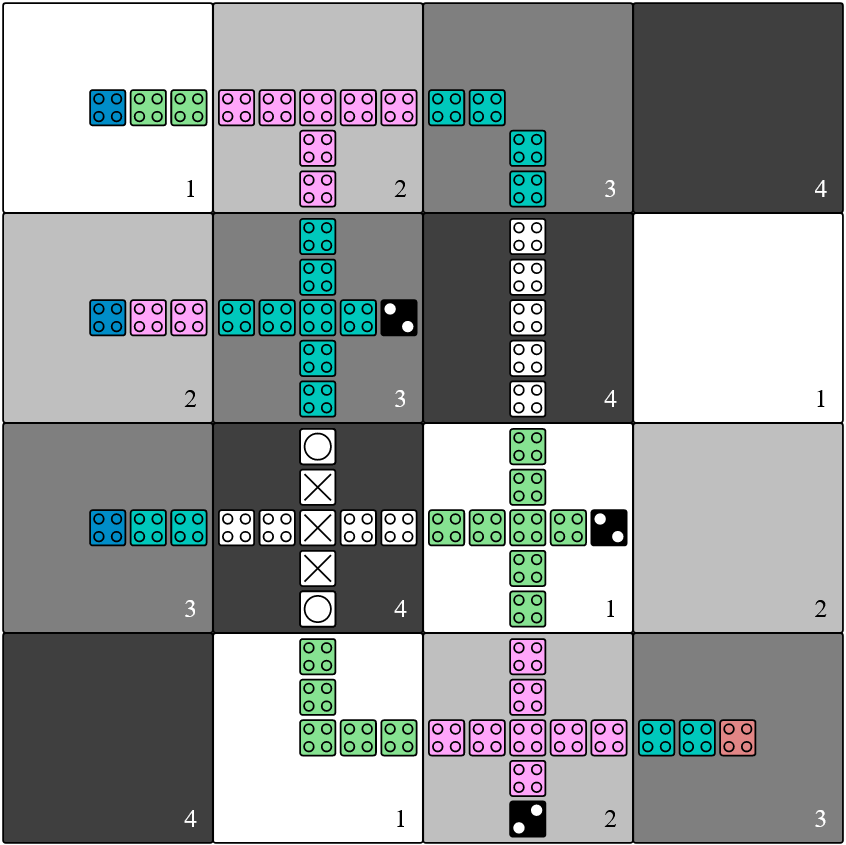
\includegraphics[scale=0.5]{input_network_mux_21}
	\caption{Placement and routing of a 2:1 mux network using the ortho algorithm with the ordering distribution network}\label{fig:input_network_mux_21}
\end{figure}

In addition to fan-out gates, issues related to inverter nodes also arise in the network design. For example, if an inverter node is assigned $south$, such as after a fan-out node, and it is intended to be placed in the same row as a primary input, a conflict arises because the input always has to wire in the x-direction. To minimize conflicts, all inverters colored $south$ must be placed at a minimum of one row further than the most southern primary input.

To further reduce the number of inverters in the logic network and prevent excessive overhead, a balancing network is introduced. This network aims to reduce the number of inverters by substituting them with fan-out nodes. For instance, in some cases a fan-out node has two inverters connected to its outgoing edges. These inverters can be replaced by a single inverter as the incoming node to the fan-out, resulting in an overall lower number of inverter nodes.

Figure \ref{fig:input_network_mux_21} shows the placement and routing of the ortho algorithm after implementing the proposed ordering distribution network. The ordering of the inputs puts first the fan-out node and then the two connected primary inputs. Since the inverter is part of the ordering distribution network it gets colored $east$ and allows the AND gates connected to the PIs to be colored south and the new rule for placement and routing can be applied. The last OR gate is not part of the distribution network and is therefore placed after the normal rules of the ortho algorithm. In the comparison to the layout in figure \ref{fig:ortho_mux_21} can be quickly seen that the resulting layout saves up place and even wire crossings. The exact results are presented and analyzed in the next chapter.

\section{Majority Gate Distribution Network}\label{sec:majgatedisnet}
This section addresses the placement and routing of majority gates in QCA circuits using the ortho algorithm. The use of majority gates is significant in QCA as they can implement the majority function using only one gate, unlike in CMOS circuits which require multiple gates, as defined in Definition \ref{Def:majf}. However, this theoretical advantage can only be realized through efficient placement and routing. To this end, a majority gates distribution network for the orthogonal algorithm is proposed, allowing for the placement and routing of majority gates and enabling a comparison of design metrics between a logic network in the MIG representation and its corresponding logic network in the AIG representation

\subsection{The proposed signal distribution Network}

\begin{figure}
	\centering
	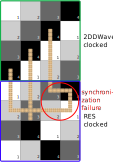
\includegraphics[scale=0.5]{Timing_failure_RES}
	\caption{Global sychronization violation when connecting 2DD-Wave and RES clocked scheme}\label{fig:Timing_failure_RES}
\end{figure}

The orthogonal algorithm uses 2DDWave clocking, which limits the direction assignment to only two options, $east$ and $south$, and can only handle the placement and routing of 2-input logic gates. To introduce "+"-majority gates into the layout, a RES-like clocking scheme is necessary, which includes tiles with three incoming tiles and one outgoing tile. As shown in Figure \ref{subfig:RES}, such a tile is located at position $(1, 1)$ and is suitable for placing a "+" majority gate, allowing it to be connected with three incoming signals. However, changing the clocking scheme of ortho to RES would be highly inefficient and difficult to implement. This is because if the clocking were completely changed to RES, the algorithm would not be able to utilize every row and column of the clocking. The RES scheme supports signals to flow into the western or northern directions, thus only the first and third rows and the second and fourth columns support eastern and southern signal propagation. This would lead to only these parts of the clocking being utilized for the placement of two-input gates, resulting in approximately double the area usage for only two-input logic gates.
An alternative approach to utilizing the RES scheme is to only support it in certain evenly distributed regions, allowing majority gates to be placed in specific, permanently assigned locations. For example, the layout could be divided into $4x4$ tile sub-regions, and every fifth sub-region would be RES clocked, while the rest would be occupied with the 2DDWave scheme. On one hand, this approach should not produce as much area overhead since only some regions are inaccessible for two-input logic gates. However, the permanent clocking assignment limits the placement of majority gates to specific spots, leading to large area overhead if a majority gate needs to be placed far away from such a sub-region. For a network consisting mainly of majority gates, this implementation would also waste most of the 2DD-Wave clocked area. Another aspect to consider is the trivial global synchronization constraints within a uniformly 2DDWave clocked layout, which are disrupted by introducing RES clocking within the layout. By introducing irregular clocking such as RES sub-regions, signals can pass different amounts of tiles to reach the same tile, thereby violating the global synchronization constraint. In Figure \ref{fig:Timing_failure_RES}, the top four rows are 2DD-Wave clocked and the bottom four rows are RES clocked. In the 2DD-Wave scheme, all three paths start globally synchronized. The two left paths need exactly one clock cycle to reach the majority gate. However, the right path in the RES scheme causes a delay, so that the signal travels two clock cycles before reaching the majority gate, thereby violating the global synchronization constraint.

%On the other hand, for the placement of three input majority gates a new direction assignment would have to be introduced to the logic network, since one signal would need a direction assignment $west$, changing the theory and complexity underlying the ortho algorithm.

\begin{figure}
	\centering
	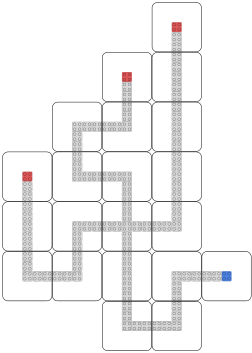
\includegraphics[scale=0.3]{Majority_Distribution_network}
	\caption{Proposed majority gate distribution network}\label{fig:QCA_Maj_nw}
\end{figure}


To overcome these complications, the proposed distribution network uses a custom clocking scheme only in areas where majority gates are placed, and addresses the global signal synchronization constraint. As a result, the placement and routing of solely two-input gates should not produce any additional area overhead. Figure \ref{fig:QCA_Maj_nw} illustrates the proposed majority gate signal distribution network, which is integrated into the orthogonal algorithm. The red-marked cells indicate the three inputs for the majority gate distribution network. The cells in the middle of the tile are marked because they can be connected from above north or the west, which would result in one normal wire and one bent wire. The output in blue allows the algorithm to wire it in the east or south direction, eliminating any limitations. It is also important to note that the input tiles as well as the output tiles have the same clocking number as in a regular 2DDWave scheme, allowing for straightforward connections. Although the proposed distribution network does not produce any area overhead for the placement and routing of two-input gates, it can be seen that it does produce excess area due to its complex wiring, resulting from the synchronization conditions that had to be considered in its design. In comparison to the implementation of an AIG representation of the majority function designed with the orthogonal algorithm, the placement and routing of this single majority gate already needs more area. However, it should be noted that no wire crossings are used. Assuming that wire crossings have a high cost, the proposed majority gate distribution network is considered more ideal, although a meaningful cost comparison of the two implementations can only be done under a cost function that represents wire crossings in terms of normal gates.

The design constraints used to develop the signal distribution network are discussed in the following. Firstly, the distribution network should not contain any wire-crossings as they are considered highly costly. While introducing a cost-metric for wire-crossings may result in a more efficient implementation, this work excludes wire-crossings as a design rule for the network. Secondly, the distribution network must meet the global synchronization constraint. In a 2DDWave clocked layout, every diagonal is synchronous, and every signal wired on the same diagonal passes the same number of tiles following the orthogonal placement and routing. However, when examining the incoming tiles of a three-input tile, it can be seen that only two of the incoming tiles are on the same diagonal, and the third one is shifted by half a clock cycle. This results in the third incoming signal being delayed by half a clock cycle, violating the global synchronization constraint. Additionally, signals must pass a multiple of whole clock cycles in the signal distribution network in order to support the further use of 2DDWave and the local synchronization constraint. To satisfy this, the initially synchronous signals are first delayed by half a clock signal at the tile where the majority gate is placed, meeting the global synchronization constraint. Then, the output signal of the majority gate is delayed by another half a clock cycle, allowing it to be connected to the regular 2DDWave clocking scheme used in the remaining layout. The delays resulting from the distribution network lead to a total delay of one whole clock cycle for the signal propagating through the majority gate distribution network compared to all other signals in the logic network. Because the delay affects the global synchronization constraint, it has to be considered for each gate connected to the parents of a majority gate distribution network. In the following, the basic placement and routing of the majority gates distribution network and the insertion of buffers in order to meet global synchronization is discussed.

\subsection{Placement and routing}

\begin{figure}
	\centering
	\begin{tikzpicture}[node distance={2cm and 2cm}, thick, main/.style = {draw, rectangle}] 
		\node[fit={(0,0) (8, 8)}, inner sep=0pt, draw=black, thick] (frame) {};
		\node[fit={(1,0) (7, 8)}, inner sep=0pt, draw=black, thick, fill=lightgray] (wires) {};
		\node[fit={(1,5) (3, 8)}, inner sep=0pt, draw=black, thick, fill=cyan] (logic) {C. logic \\ w/o MAJ};
		\node[fit={(3,4) (4, 5)}, inner sep=0pt, draw=black, thick, fill=yellow] (logic) {MAJ};
		\node[fit={(4,3) (5, 4)}, inner sep=0pt, draw=black, thick, fill=cyan] (logic) {};
		\node[fit={(5,2) (6, 3)}, inner sep=0pt, draw=black, thick, fill=yellow] (logic) {MAJ};
		\node[fit={(6,0) (7, 2)}, inner sep=0pt, draw=black, thick, fill=cyan] (logic) {};
		
		\node[fit={(0,6.5) (1, 8)}, inner sep=0pt, draw=black, thick, fill=TUMGray] (PIs) {PIs};
		\node[fit={(7,0) (8, 8)}, inner sep=0pt, draw=black, thick, fill=TUMGray] (POs) {POs};
		
		
		
		\draw (3.5,1) node [align = left] {Area for wiring \\ and buffer insertion};
		
		
	\end{tikzpicture} 
	\caption{Scheme of the P\&R using the Majority Gate Distribution Network} \label{fig:majority_scheme}
\end{figure}

The placement and routing of the proposed signal distribution network are subject to certain constraints. Firstly, the coloring of majority gates must be reviewed, as the logic network now includes three input nodes. However, the coloring algorithm can include helping nodes to resolve coloring conflicts of edges, and therefore, by dividing every edge with a helping node, it can be seen that a trivial coloring can be found even when including three input nodes in the logic network. Another aspect to consider is the need for a new direction to connect a third signal to the majority gate. However, since the only time such wiring occurs is inside the fixed distribution network, which can be placed and routed in the usual south-eastern manner, no additional directions need to be included. Additionally, the irregular clocking inside the signal distribution network must be reviewed. These irregularities don't allow the algorithm to wire connections over the network, requiring a special treatment for the placement of the majority gates. From the algorithm's perspective, a majority gate cannot be placed just south or east of another gate, as these gates could need wiring through the majority gate distribution network. Instead, the algorithm is forced to always assign the majority gate distribution network to the south and east direction to prevent routing conflicts. This means that for majority gates, a trivial coloring is always chosen. The major drawback of this is that the area is not used optimally and the layout is extended in two directions as shown in Figure \ref{fig:majority_scheme}, compromising the beneficial use of the "+" majority gate.

\subsection{Signal synchronization and buffer insertion}
The placement and routing using the proposed distribution network results in a delay of one clock cycles of signals passing through a majority gates. Since the tile-based clocking doesn't support a speedup of a signal, every other signal which comes into contact with a delayed signal also has to be delayed in order to meet the global synchronization constraint. Therefore a function is introduced to compute the delay of signals and allowing signals which are connected together to be synchronized by buffer insertion. For the delay computation, the algorithms views every incoming edge from every node starting at the primary output. If an incoming edge is connected to a majority gate, every other incoming edge of the same node gets a delay of one assigned, if this edge is not also connected to a majority gate. In the latter case all incoming edges of a node are delayed, resulting again in synchronous behavior. Nodes with incoming edges from majority gates are marked as delayed and the delays stack for every majority gate on a path. The inserted delays then result from the difference of delays of the incoming edges from a node and are realized by inserting wire buffers. 

\begin{figure}
	\centering
	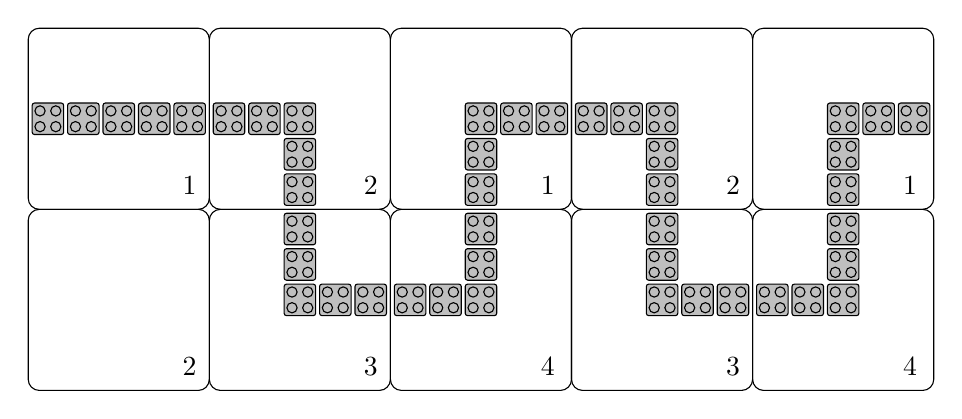
\begin{tikzpicture}
		\begin{scope}[xshift=-2.3cm, rotate=90]
			\draw[rounded corners] (-0.05, -0.1 - 0.85) rectangle (2.3-0.05, 2.3-0.1 - 0.85){};
			
			\foreach \x/\y in {0.9/0.9, 0.9/0.45, 0.9/0, 0.9/-0.45, 0.9/-0.9}
			{
				\draw[rounded corners = 0.3mm, fill=lightgray] (\x, 0 + \y) rectangle (1.2/3 + \x, 1.2/3 + \y){};
				\draw (0.3/3+ \x,0.3/3 + \y) circle (0.65mm);
				\draw (0.9/3+ \x,0.3/3+ \y) circle (0.65mm);
				\draw (0.3/3+ \x,0.9/3 + \y) circle (0.65mm);
				\draw (0.9/3+ \x,0.9/3 + \y) circle (0.65mm);
			}
			\node[text=black] (A1) at (0.25,-0.7) {$1$};
		\end{scope}
		\begin{scope}[xshift=-2.3cm, yshift=-2.3cm, rotate=90]
			\draw[rounded corners] (-0.05, -0.1 - 0.85) rectangle (2.3-0.05, 2.3-0.1 - 0.85){};
			
			\node[text=black] (A1) at (0.25,-0.7) {$2$};
		\end{scope}
		\begin{scope}[shift={(0, 0)}, rotate=90]
			\draw[rounded corners] (-0.05, -0.1 - 0.85) rectangle (2.3-0.05, 2.3-0.1 - 0.85){};
			
			\foreach \x/\y in {0.9/0.9, 0.9/0.45, 0.9/0, 0/0, 0.45/0}
			{
				\draw[rounded corners = 0.3mm, fill=lightgray] (\x, 0 + \y) rectangle (1.2/3 + \x, 1.2/3 + \y){};
				\draw (0.3/3+ \x,0.3/3 + \y) circle (0.65mm);
				\draw (0.9/3+ \x,0.3/3+ \y) circle (0.65mm);
				\draw (0.3/3+ \x,0.9/3 + \y) circle (0.65mm);
				\draw (0.9/3+ \x,0.9/3 + \y) circle (0.65mm);
			}
			\node[text=black] (A1) at (0.25,-0.7) {$2$};
		\end{scope}
		\begin{scope}[xshift=3.2cm, yshift=1.3cm, rotate=180]
			\draw[rounded corners] (-0.05, -0.1 - 0.85) rectangle (2.3-0.05, 2.3-0.1 - 0.85){};
			
			\foreach \x/\y in {0.9/0.9, 0.9/0.45, 0.9/0, 0/0, 0.45/0}
			{
				\draw[rounded corners = 0.3mm, fill=lightgray] (\x, 0 + \y) rectangle (1.2/3 + \x, 1.2/3 + \y){};
				\draw (0.3/3+ \x,0.3/3 + \y) circle (0.65mm);
				\draw (0.9/3+ \x,0.3/3+ \y) circle (0.65mm);
				\draw (0.3/3+ \x,0.9/3 + \y) circle (0.65mm);
				\draw (0.9/3+ \x,0.9/3 + \y) circle (0.65mm);
			}
			\node[text=black] (four) at (0.25 ,1.05) {$1$};
		\end{scope}
		\begin{scope}[xshift=-0.4cm, yshift=-0.1cm, rotate=270]
			\draw[rounded corners] (-0.05, -0.1 - 0.85) rectangle (2.3-0.05, 2.3-0.1 - 0.85){};
			
			\foreach \x/\y in {0.9/0.9, 0.9/0.45, 0.9/0, 0/0, 0.45/0}
			{
				\draw[rounded corners = 0.3mm, fill=lightgray] (\x, 0 + \y) rectangle (1.2/3 + \x, 1.2/3 + \y){};
				\draw (0.3/3+ \x,0.3/3 + \y) circle (0.65mm);
				\draw (0.9/3+ \x,0.3/3+ \y) circle (0.65mm);
				\draw (0.3/3+ \x,0.9/3 + \y) circle (0.65mm);
				\draw (0.9/3+ \x,0.9/3 + \y) circle (0.65mm);
			}
			\node[text=black] (A1) at (1.1+0.85,1.1) {$3$};
		\end{scope}
		\begin{scope}[xshift=1cm, yshift=-1.4cm, rotate=0]
			\draw[rounded corners] (-0.05, -0.1 - 0.85) rectangle (2.3-0.05, 2.3-0.1 - 0.85){};
			
			\foreach \x/\y in {0.9/0.9, 0.9/0.45, 0.9/0, 0/0, 0.45/0}
			{
				\draw[rounded corners = 0.3mm, fill=lightgray] (\x, 0 + \y) rectangle (1.2/3 + \x, 1.2/3 + \y){};
				\draw (0.3/3+ \x,0.3/3 + \y) circle (0.65mm);
				\draw (0.9/3+ \x,0.3/3+ \y) circle (0.65mm);
				\draw (0.3/3+ \x,0.9/3 + \y) circle (0.65mm);
				\draw (0.9/3+ \x,0.9/3 + \y) circle (0.65mm);
			}
			\node[text=black] (four) at (1.95 ,-0.65) {$4$};
		\end{scope}
		
		\begin{scope}[xshift=4.6cm, yshift=0cm, rotate=90]
			\draw[rounded corners] (-0.05, -0.1 - 0.85) rectangle (2.3-0.05, 2.3-0.1 - 0.85){};
			
			\foreach \x/\y in {0.9/0.9, 0.9/0.45, 0.9/0, 0/0, 0.45/0}
			{
				\draw[rounded corners = 0.3mm, fill=lightgray] (\x, 0 + \y) rectangle (1.2/3 + \x, 1.2/3 + \y){};
				\draw (0.3/3+ \x,0.3/3 + \y) circle (0.65mm);
				\draw (0.9/3+ \x,0.3/3+ \y) circle (0.65mm);
				\draw (0.3/3+ \x,0.9/3 + \y) circle (0.65mm);
				\draw (0.9/3+ \x,0.9/3 + \y) circle (0.65mm);
			}
			\node[text=black] (A1) at (0.25,-0.7) {$2$};
		\end{scope}
		\begin{scope}[xshift=7.8cm, yshift=1.3cm, rotate=180]
			\draw[rounded corners] (-0.05, -0.1 - 0.85) rectangle (2.3-0.05, 2.3-0.1 - 0.85){};
			
			\foreach \x/\y in {0.9/0.9, 0.9/0.45, 0.9/0, 0/0, 0.45/0}
			{
				\draw[rounded corners = 0.3mm, fill=lightgray] (\x, 0 + \y) rectangle (1.2/3 + \x, 1.2/3 + \y){};
				\draw (0.3/3+ \x,0.3/3 + \y) circle (0.65mm);
				\draw (0.9/3+ \x,0.3/3+ \y) circle (0.65mm);
				\draw (0.3/3+ \x,0.9/3 + \y) circle (0.65mm);
				\draw (0.9/3+ \x,0.9/3 + \y) circle (0.65mm);
			}
			\node[text=black] (four) at (0.25 ,1.05) {$1$};
		\end{scope}
		\begin{scope}[xshift=4.2cm, yshift=-0.1cm, rotate=270]
			\draw[rounded corners] (-0.05, -0.1 - 0.85) rectangle (2.3-0.05, 2.3-0.1 - 0.85){};
			
			\foreach \x/\y in {0.9/0.9, 0.9/0.45, 0.9/0, 0/0, 0.45/0}
			{
				\draw[rounded corners = 0.3mm, fill=lightgray] (\x, 0 + \y) rectangle (1.2/3 + \x, 1.2/3 + \y){};
				\draw (0.3/3+ \x,0.3/3 + \y) circle (0.65mm);
				\draw (0.9/3+ \x,0.3/3+ \y) circle (0.65mm);
				\draw (0.3/3+ \x,0.9/3 + \y) circle (0.65mm);
				\draw (0.9/3+ \x,0.9/3 + \y) circle (0.65mm);
			}
			\node[text=black] (A1) at (1.1+0.85,1.1) {$3$};
		\end{scope}
		\begin{scope}[xshift=5.6cm, yshift=-1.4cm, rotate=0]
			\draw[rounded corners] (-0.05, -0.1 - 0.85) rectangle (2.3-0.05, 2.3-0.1 - 0.85){};
			
			\foreach \x/\y in {0.9/0.9, 0.9/0.45, 0.9/0, 0/0, 0.45/0}
			{
				\draw[rounded corners = 0.3mm, fill=lightgray] (\x, 0 + \y) rectangle (1.2/3 + \x, 1.2/3 + \y){};
				\draw (0.3/3+ \x,0.3/3 + \y) circle (0.65mm);
				\draw (0.9/3+ \x,0.3/3+ \y) circle (0.65mm);
				\draw (0.3/3+ \x,0.9/3 + \y) circle (0.65mm);
				\draw (0.9/3+ \x,0.9/3 + \y) circle (0.65mm);
			}
			\node[text=black] (four) at (1.95 ,-0.65) {$4$};
		\end{scope}
		
	\end{tikzpicture}
	\caption{Buffer in $east$ direction with resolve column and respective clocking}\label{fig:QCA_buf}
\end{figure}

Figure \ref{fig:QCA_buf} depicts a buffer in the east direction, which can also be used in the south direction by just rotating it 90 degrees. The snake-shaped structure delays a signal by exactly one clock cycle and is also used in custom placement and routing resulting from the QCA ONE library \cite{QCA_scl}. As in the majority gate distribution network, the buffers support irregular clocking, creating zones through which the algorithm cannot wire. In the case of buffers only one column or row is made impassable, allowing them to be tracked and introducing a rewiring for conflicts. Algorithm \ref{alg:majority_network} shows the code snippets which are changed and added to ortho in order to allow the placement and routing of majority gates distribution networks and the corresponding majority buffers. Figure \ref{fig:majority_with_buf} shows the placement of a majority gate inside the input distribution network and two and gates that have to be delayed to be connected to the delayed signal coming out of the majority gate distribution network. The insertion of the first buffer blocks the eastern direction of the second input. For this case, a resolve column is introduced where the signal can be assigned to a new row and be wired without conflict. From this layout, it can already be seen that the implementation of the majority gate distribution network brings several complications with it, all resulting in area overhead, which stands in contrast to the area which should be saved by introducing majority gates in the first place.

\begin{algorithm}[H]
	\vdots
	
	\begin{algorithmic}
		\State Convert $N$ to a 3-graph by substitution and balance inverters at fan-out nodes, except for majority gates
		\State Compute the delay as majority buffer insertion $buf_{maj}$ for every node and assign it to the incoming signals $\sigma$
		\State Order primary input nodes
		\State Create vectors with from the majority buffers blocked columns $bl_c$ and rows $bl_r$
		\State \vdots
		\ForAll {vertex $v_1, ..., v_i \in N $ with at most three incoming signals $\sigma_1, \sigma_2, \sigma_3$}
		\State Rewire incoming signals which are wired on $bl_c$ or $bl_r$
		\State \vdots
		\If{vertex $v$ has fanin of three (is a majority gate)}
		\If{$d(\sigma_1) = d(\sigma_2) = d(\sigma_3) = south$}
		\State{Extend $L$ by one row and wire the incoming signal to $(w_p, h-1)$ for every incoming signal}
		\EndIf
		\State Insert majority buffers according to the delay computed in $buf_{maj}$ and safe blocked columns $bl_c$ and rows $bl_r$
		\State Extend the layout by number of rows $(7)$ and columns $(5)$ of the majority gate distribution network and place the distribution network at $(w-5, h-7)$
		\State Connect incoming signals west to the inputs of the distribution network
		\ElsIf{$d(\sigma_1) = d(\sigma_2) = east$}
		\State Insert majority buffers according to the delay computed in $buf_{maj}$ and safe blocked rows $bl_r$
		\State \vdots
		\ElsIf { signals are labeled $south$}
		\State Insert majority buffers according to the delay computed in $buf_{maj}$ and safe blocked columns $bl_c$
		\State \vdots
		\EndIf
		
		\EndFor
%		\State \vdots \\
%		\Return $L$
	\end{algorithmic}
	\caption{Ortho changes with majority gate distribution network}\label{alg:majority_network}
\end{algorithm}

\begin{figure}
	\centering
	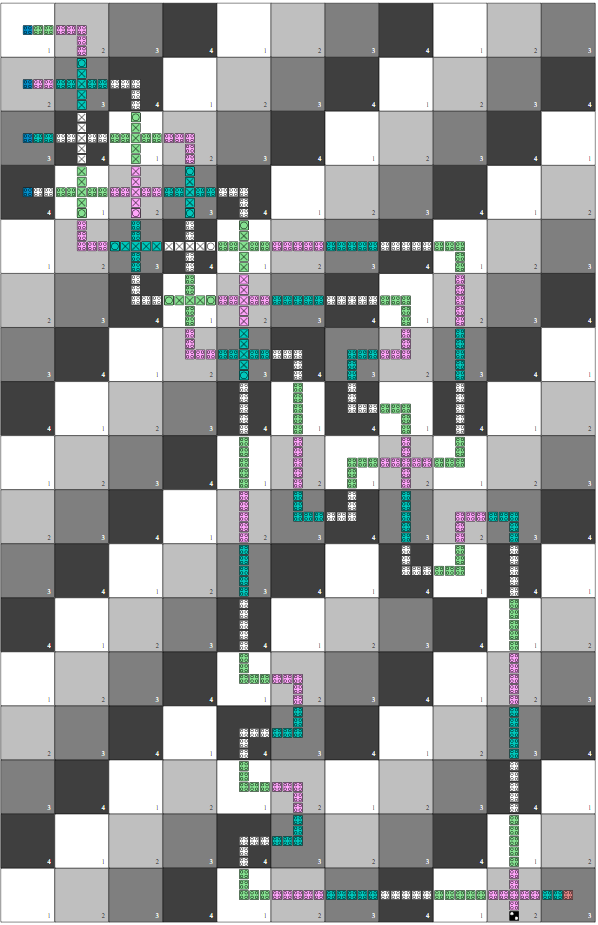
\includegraphics[scale=0.65]{maj_example}
	\caption{Placement and routing of a majority gate in conjunction with a delayed primary input}\label{fig:majority_with_buf}
\end{figure}


\section{Sequential Distribution Network}
In this section, a distribution network that enables orthogonal automatic design of sequential circuits is presented. To the authors' knowledge, there is currently no solution for placing and routing sequential circuits in Quantum-dot Cellular Automata (QCA). The existing algorithms for handling sequentiality in QCA, discussed in Chapter \ref{chapter:SotA}, simply translate CMOS structures into QCA and rely on an external clock signal, which is considered unnatural in the context of QCA's inherent clocking paradigm. The proposed placement and routing method utilizes the concept of signal-delaying wires from \cite{Walter}, and builds upon it to enable automated placement and routing.

\subsection{Placement and Routing}
Before looking at the algorithm, first the idea of an FF wire should be discussed in the domain of placement and routing and not only as a single element. From the FF wire it can be examined that the proposed FF implementation requires more complex clock generators for every FF, and it is not sure if this is possible to implement. Also if we look back at the analogy of CMOS, a sequential circuit includes a combinational logic block and the storage element, which is formed by a wire FF in this case. But there is still a big difference. While in CMOS the information can just be arbitrarily wired back from the storage to the inputs of the combinational logic, in QCA the wiring back implies the placement of wire segments of which each is delaying the information by one clocking zone already, being a partial FF. If a signal is wired through four adjacent wire gates, a basic FF is already formed, since the information is delayed by four clock zones equaling a clock cycle. When looking back to the functionality of a storage element, it can be found that this delay is exactly the purpose of a clocking element and the reason why the clocking for the wire FF is customized. The idea proposed in this work is now to use the delay, which occurs naturally due to sequential wiring to mimic storage elements and therefore wire segments can be summarized to FFs without the need for customized clocking. 

\begin{figure}
	\centering
	\begin{tikzpicture}[node distance={2cm and 2cm}, thick, main/.style = {draw, rectangle}] 
		\node[fit={(0,0) (8, 8)}, inner sep=0pt, draw=black, thick] (frame) {};
		\node[fit={(2,2) (6, 8)}, inner sep=0pt, draw=black, thick, fill=cyan] (logic) {Combinational logic};
		\node[fit={(0,6.5) (1, 8)}, inner sep=0pt, draw=black, thick, fill=TUMGray] (PIs) {PIs};
		\node[pattern=north west lines, pattern color=TUMGray, fit={(1,6.5) (2, 8)}, inner sep=0pt, draw=black, thick] (wires) {wires};
		\node[fit={(1,5) (2, 6.5)}, inner sep=0pt, draw=black, thick, fill=lightgray] (ROs) {ROs};
		\node[pattern=north west lines, pattern color=TUMGray,fit={(6,3.5) (7, 8)}, inner sep=0pt, draw=black, thick] (wires) {wires};
		\node[fit={(7,3.5) (8, 8)}, inner sep=0pt, draw=black, thick, fill=TUMGray] (POs) {POs};
		\node[fit={(6,2) (7, 3.5)}, inner sep=0pt, draw=black, thick, fill=lightgray] (RIs) {RIs};
		
		\draw[] (7, 3.5) -- (8, 3.5);
		\draw[] (0, 6.5) -- (1, 6.5);
		\draw[fill=Apricot] (0, 0) -- (0, 6.5) -- (1, 6.5)  -- (1, 5) -- (2, 5) -- (2, 2) -- (7, 2) -- (7, 3.5) -- (8, 3.5) -- (8, 0) -- (0, 0);
		\draw (4,1) node [align=left] {Sequential wires from Ris to Ros \\ with delay of $c$ clock cycles};
		%		\draw[->] (2) -- (5);
		%		\draw[->] (3) -- (6);
		%		\draw[->] (4) -- (6);
		%		\draw[->] (5) -- (7);
		%		\draw[->] (6) -- (7);
		%		\draw[->] (7) -- (f);
		
	\end{tikzpicture} 
	\caption{Scheme of a sequential circuit layout after placement and routing} \label{fig:sequential_gate_sample}
\end{figure}

Considering the placement and routing of sequential circuits, not only a distribution network has to be designed but also the logic network has to be expanded regarding to storage elements. They are represented in the logic network by registers with its corresponding input, determining the value, which has to be stored, and its output, which gives the register value to the combinational logic again after delaying it to the next \textit{circuit clocking cycle}. A circuit clocking cycle refers to one cycle of Bennet clocking that has propagated through the circuit completely. The registers are implemented into the logic network as follows. Register inputs (RIs) are treated similar to primary outputs, therefore they are dangling edges, which point to no node but additionally have a register output assigned. Register outputs (ROs) are treated similarly to primary inputs, being terminal vertices, but always feeding in the data which were given to the corresponding register input in the last circuit clocking cycle. Therefore, the logic network extends to $N = (\Lambda, I, RO, \Sigma, O, RI)$. Here it has to be mentioned that for the input distribution network due to their similarity ROs can be treated just like PIs, enabling the combination with the sequential distribution network.
Also, for placement and routing, the similarities between PIs/ROs and POs/RIs can be exploited. The schematic layout resulting from the described algorithm is shown in figure \ref{fig:sequential_gate_sample}. When the first part of ortho is performed, first the combinational logic part is placed and routed, treating ROs just like PIs and RIs just like POs. From this stage, a routing from the RIs to the ROs has to be found, which retains the local and global synchronization constraint. Because every register input has exactly one register output assigned, first of all, the register inputs are rewired and sorted in the same order as the register outputs. The ordering follows in a way that all RIs are put on a diagonal, and since to this point every gate is clocked uniformly with 2DDWave, the signals are all synchronized. With this starting position now wires with the same length have to be found between every register input and output. Since the wires now also have to go in western and northern directions in order to close the loop between the ROs in the upper left corner and the RIs in the down-right corner of the layout, the wiring is not arbitrary. One big issue is also that the clocking cannot be chosen independently for each back-loop because the loops cross each other. Also another issue regarding timing can be derived. Considering a primary Input in a completely combinational circuit being placed in the fifth row of the layout. In this case the PI is set in a different \textit{time zone}, because its signal is globally delayed by one clock cycle. Until now the assumption was made, that an input network can be used to delay the primary input by one clocking cycle to achieve again global synchronization. When an RO is placed in a different time zone, this also has to be respected by the wiring of the registers. As already mentioned, the registers do not delay the information by only one clocking cycle but by multiple clocking slowing down the performance of the circuit drastically. This huge delay is due to the fact that ortho lays the combinational logic only in the south-eastern direction, always increasing the distance between PIs/ROs and POs/RIs. Therefore the sequential signal distribution network always grows with the size of the combinational logic.\\
Maybe a folding operation can be found for the ortho algorithm so that the distance between RIs and ROs can be decreased and therefore the delay produced by the sequential distribution network can be decreased as well.

\begin{algorithm}[H]
	\vdots
	
	\begin{algorithmic}
		\If{vertex $v$ is primary input}
		{
			\State Extend $L$ by one row
			\State Place v at position $(0, h - 1)$
			\State Wire the primary input to position $(num_{reg}*2, h - 1)$ 
			\If{vertex $v$ is colored $south$}
			\State Extend $L$ by one column
			\State Wire the primary input to position $(w - 1, h - 1)$ 
			\EndIf
		}
		\ElsIf{vertex $v$ is register output}
		{
			\State Extend $L$ by one row
			\State Place v at position $(num_{reg}*2, h - 1)$
			\If{vertex $v$ is colored $south$}
			\State Extend $L$ by one column
			\State Wire the primary input to position $(w - 1, h - 1)$ 
			\EndIf
		}
		\State\vdots
		\EndIf
		\State Connect the primary outputs to the respective borders
		\State Connect the register inputs to the respective borders and connect the RIs to the ROs
		\Return $L$
		
		
	\end{algorithmic}
	\caption{Ortho changes with sequential distribution network}\label{alg:seq_network}
\end{algorithm}

\subsection{RAM cell}
As mentioned in \ref{subsec:RAM_SoA}, a RAM cell can be realized using wire delays to safe the data and a MUX, which can input new data into the RAM cell. With the possibility of placing and routing sequential circuits a RAM cell now is a MUX with two PIs and one RO. The PIs are the BL and WL, while the RO is the information held in the RAM cell. The output of the MUX is both the PO and the RI.
Figure \ref{fig:QCA_RAM} shows a RAM cell, with its respective wordline(s), bitline(s) and latch. The core of the cell is a latch, which is simply propagating the data in a circle and therefore producing a stable output once in every clock cycle. The input mechanism works via two majority gates. The majority gates with the wordlines decides if $BL$ or $\bar{BL}$ should be propagated to the majority gate connected to the loop. When $WL_1=\bar{WL_2}$ the majority gate always outputs the third input $BL$. But for $WL_1=WL_2=\bar{BL}$ the first majority gate outputs $\bar{BL}$.
If the first majority gate has as output $BL$, the second majority gate has $BL$ twice as input and overrides the data in the RAM cell. If the first majority gate has as output $\bar{BL}$, the second majority gate has two distinct inputs and the data which is held in the cell. In this case the stored bit always decides the output and therefore it is latched meaning that the data is stored. For the read operation only one majority gate is needed and in order to read the RAM cell the output-wordlines have to be inverted. Otherwise if both output-worlines are set to "0", the output isn't read. The corresponding truth tables for the RAM cell is shown in \ref{fig:QCA_RAM}.
\begin{figure}
	\centering
	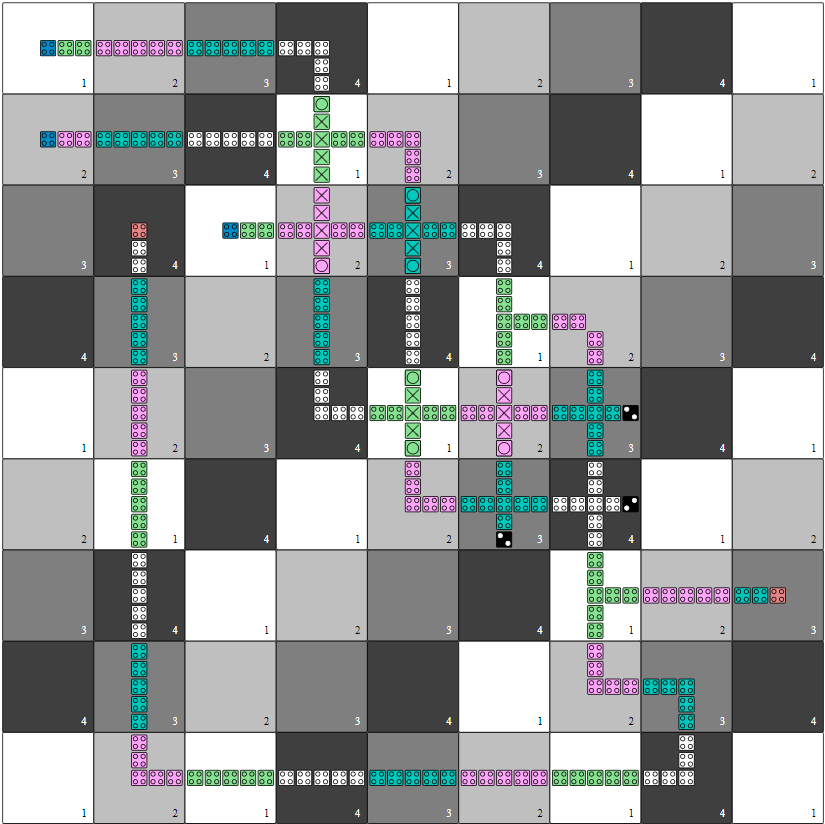
\includegraphics[scale=0.4]{mux21_seq}
	
%	\subfigure[Truth table]
%	{
%		% Table generated by Excel2LaTeX from sheet 'Tabelle1'
%		\centering
%		\begin{tabular}{cllll}
%			& Input1 & Input2 & Input3 & Output \\
%			\multirow{2}[0]{*}{Maj1} & $WL_1$   & $WL_2=\overline{WL_1}$ & $BL$    & $BL$ \\
%			& $WL_1=\overline{BL}$ & $WL_2=\overline{BL}$ & $BL$    & $\overline{BL}$ \\
%			\multirow{2}[0]{*}{Maj2} & $X$     & $BL$    & $BL$    & $BL$ \\
%			& $X$     & $\overline{BL}$ & $BL$    & $X$ \\
%		\end{tabular}%
%		\label{subfig:QCA_RAM_tt}
%	}
	\caption{QCA RAM cell designed as 2:1 mux with a sequential distribution network}\label{fig:QCA_RAM}
\end{figure}